\documentclass[11pt, english]{article}

\usepackage[english]{babel}
\usepackage[T1]{fontenc}
\usepackage{graphicx}
\usepackage{wrapfig}
\usepackage{lipsum}
%\usepackage{titlesec}
\usepackage{caption}
\usepackage{subcaption}
\usepackage{hyperref}
\usepackage{float}
\usepackage{cite}
\usepackage[bitstream-charter]{mathdesign}
\usepackage{siunitx}
\usepackage{color}
\usepackage{setspace}
\usepackage[usenames,dvipsnames,svgnames,table]{xcolor}
\usepackage[toc, acronym]{glossaries}
\makeglossaries
\hypersetup{
        colorlinks = true,
        citecolor = darkgray
}
\usepackage{geometry}
\geometry{
        a4paper,
        total={170mm,257mm},
        left=20mm,
        top=20mm,
}


\begin{document}
\hypersetup{linkcolor=darkgray}

\begin{titlepage}
\hypersetup{pageanchor=false}
    \begin{center}
        \vspace*{1cm}
        \Huge
	\par\noindent\rule{\textwidth}{0.4pt} \\ ~ \\
	Developing a Fishing Risk Framework from Satellites and Ocean Data \\
        \par\noindent\rule{\textwidth}{0.4pt} \\ ~ \\
        \huge
        \textbf{\textsc{White Paper}} \\
        \vspace{5cm}
        
\includegraphics[width=0.8\textwidth]{images/logo} \\
        \vspace{2cm}
	\Large
	\textbf{\textsc{Date last modified:}} \\
        \today \\
        \vfill
	\Large
	\textbf{\textsc{Authors:}} \\
	William \textsc{Grimes} \hfill
	Iv\'{a}n \textsc{Higuera-Mendieta} \hfill
	Shubham \textsc{Tomar} \\~\\~\\
	\begin{minipage}{0.485\textwidth}
		\begin{flushleft}
			\Large
			\textbf{\textsc{Project Manager:}} \\
			Paul \textsc{Van der Boor}
		\end{flushleft}
	\end{minipage}
	~
	\begin{minipage}{0.485\textwidth}
		\begin{flushright}
			\Large
			\textbf{\textsc{Technical Mentor:}} \\
			Jane \textsc{Zanzig}
		\end{flushright}
	\end{minipage}
    \end{center}
\end{titlepage}

\hypersetup{pageanchor=true}


\input{sections/glossary} % glossary
%\input{sections/acronyms} % acronyms

\begin{abstract}
\doublespacing
\noindent The lack of traceability within the fishing industry limits responsible governance, and management of the oceans. As a consequence of this lack of traceability illegal, unregulated and unreported fishing is rife, affecting fisheries worldwide. A major challenge within fish traceability is determining whether fish have been caught sustainably from vessels acting in a legal, and responsible manner. The proof-of-concept system proposed here creates a vessel risk framework to assess the likelihood that a vessel has engaged in illegal, unregulated, or unreported fishing.\\~\\
\noindent Using historical vessel tracking data the system first predicts the likelihood at each time point that a vessel was fishing, using features including its movement and distance from shore. Vessels that are fishing are then scored using multiple indicators to evaluate the risk of these behaviours. Indicators include the likelihood that a vessel has previously fished in a marine protected area or exclusive economic zone, and the intermittency of the vessels automatic identification system positional signal. This information is displayed in web application that allows the user to weight the components according to the use case, or for convenience combined into a unified vessel risk score.\\~\\
\noindent This proposed fishing risk framework combines multiple data sets by correlating these tracking data with satellite imagery. For all historical vessel tracking and all time points the available satellite imagery is found, this could be used as further evidence to substantiate our risk indicator. This proof-of-concept shows show how multiple data sources can be combined to start building a library of historic evidence and data of a vessels behaviour. This gives governments, retailers, coastguards and enforcement agencies the information they need to improve traceability within the fishing industry, better manage the oceans, and conduct more effective enforcement.
 % abstract
\end{abstract}

\clearpage
\tableofcontents

\newpage
\section{Introduction}
Every year around 26 million tonnes of seafood worth close to \$24 billion are extracted from the planet's oceans by illegal, unreported and unregulated (IUU) fishing. These IUU fishing techniques include: extracting fish from waters of other nations or designated marine protected areas, catching fish using illegal and ecologically damaging techniques, or under-declaring fish by transshipment at sea. Such practices are especially rife in the rich tropical waters of Southeast Asia due to the burgeoning demand in the region, and challenges of enforcement. This project sets out to address the problem of IUU fishing by correlating multiple data sources, and using data science techniques to identify vessels involved in IUU fishing.

Overfishing and IUU fishing have lead to huge declines in fish stock and some species such as tuna have declined by over 90\%. Our project partner the World Economic Forum (WEF) is committed to improving the state of the world by engaging business, political, academic, and other leaders of society to shape global, regional, and industry agendas. In particular the WEF promotes initiatives to improve ocean governance, food chain sustainability, and environmental conservation.

In partnership with the WEF this DSSG Europe project has set out to create an open-source tool combining multiple data sources to help combat IUU fishing. This proof-of-principle study of fishing in the Torres Strait aimed to demonstrate how data aggregation from sources such as satellite imagery, synthetic aperture radar (SAR) and automatic identification systems (AIS) can be correlated and used with data science methods such as object recognition and anomaly detection to aid in identification of illegal fishing. This data science approach to detecting IUU fishing could ultimately improve enforcement, guide governance, and inform policy decision making.

There are many challenges associated with detecting IUU fishing. Firstly, the world's ocean comprise the majority of the Earth's surface (71\%). This is a large area to inspect and hence the volumes of data involved are large. There are many vessels in this large area relating to commercial, leisure, or fishing activities. Systems to detect and track these vessels such as automatic identification systems (AIS) tend to be implemented nationally in vessel management systems (VMS), hence there is little standardization of the data format. Satellite data on the other hand is relatively infrequent, can be obscured by cloud cover, and may not have good coverage in the ocean. Combining these data sources can be difficult to find appropriate images and AIS data. There is also a distinct lack of high-resolution open-source data sources in this domain, due to the cost of data collection.

A socially desirable outcome for this project would be to successfully demonstrate how these data can be used to identify IUU fishing. In partnership with the WEF and organisations this can be conveyed to policy and decision makers to expand the study. A socially desirable outcome would be to improve detection of illegal fishing via these data sources, a secondary outcome of this would be to provide improved enforcement of illegal fishing, which in turn would improve regulation as it becomes harder to evade capture. The result of this would be to promote more sustainable fishing practice and environmental conservation.
 % introduction
\section{Previous work}
The first step in investigating a myriad of vessel activities including piracy, illegal maritime traffic, and IUU fishing is to find where the ships are. In the literature approaches for ship detection are described using multiple algorithms and applied to various geospatial data sources. For example, \citeA{Tello2005} uses satellite-based synthetic aperture radar (SAR) and a discrete wavelet transform to capture spectral signals of vessels in the ocean. The use of SAR data fort this task is common in the literature \cite{Margarit2009, Brusch2011, Corbane2008, Paes2010} \footnote{Most of these documents rely on the \textit{TerraSAT} project data which have a resolution up to $\approx$ 16 meters.}. The ability of the SAR sensors to capture signals even in the presence of high cloud coverage gives radar data an advantage over visible (optical) data. Nonetheless, vessel detection with SAR data has limitations for identifying small ships, limited coverage, and its automatic interpretation can be a cumbersome process \cite{Zhang2006}.  

\citeA{Corbane2010}, shows a first apporach to vessel detection using panchromatic high-resolution imagery from the SPOT-5 program. The authors used a wavelet transform, which decomposes the image according to light frecquency profiles and used a novel preprocessing approach that allows having rapid classifications compared with other algorithms. \citeA{Lebona2016} also uses optical data to track vessels, although the authors use the NASA-VIIRS nightlight data. The results of the classification algortihm are cross-validated using vessel positional AIS data, confirming the correct indetification of 5000-6000 ships per night, but is not clear if this approach is suitable to identify small targets, like fishing vessels.\footnote{VIIRS day-night band, as its predecesor, the NOAA-OLS, has a lower resolution (1 $km^{2}$ at the equator), and other problems like overglooming in the coastlines that can yield false positives. To read a comprehensive assessment of the use of nightlight data to data analysis see \citeA{Min2015}}.

Image classification is not the only approach to track vessels on the ocean. Positional messages are also used to classify ship activity. The project Global Fishing Watch for example used a labelled set of fishing vessels to classify vessels in automatic identification system (AIS) data as fishing or non-fishing, this is described in \citeA{de2016correction}. This approach relies on a reliable AIS signal, and vessels fishing illegally may not have a transponder, may switch it off, or may spoof its signal to engage in these behaviours. As such this should not be relied upon as the only approach to identify vessels. Here we have used a similar model to identify fishing vessels, but plan to incorporoate other vessel detection methods.
 % previous work
\section{Data sources}
\subsection{Automatic identification system (AIS)}
Vessel location for the period from May 2016 to June 2017  was captured using the Automatic 
Identification System (AIS) transponders installed in every vessel with a length greater or equal to 
30 meters. These transponders broadcast two types of messages. First, they transmit positional signals 
every 10 seconds, reporting GPS coordinates and navigational features of the vessel (i.e., speed, course, 
and heading). The second type of message is static and reports constant features of the ship, such as name, 
callsign, length, and destination. 

Beacons near the shores capture these messages, working as an avoiding collision system with the sea coast and 
other vessels. This makes AIS an important component of maritime security \cite{Tetreault2005}. 
Coastal receivers do not always capture AIS signals away from shore.\footnote{According to Spire, the coastal 
receivers can only capture data in an 80 kilometers range.} Nonetheless, we use satellite captured AIS signal 
provided by Spire; this allows us to retrieve vessel tracking data from all over the world, and not only from 
vessels near seashores.Some caveats arise with the use of this source. First, AIS signals fetched by satellites
can \textit{bunch together} bunch together leading to data loss, since the satellite is only able to process a 
limited number of signals at a time. Second, accuracy is not always certain. Hence there is a possible measurement 
error in the location and other features of the vessels. Lastly, there is the possibility of AIS tampering in 
vessels involved in illegal activities, such as UUI. 

\subsection{Satellite imagery}

To account for a visual validation of the AIS data, we used different sources of proprietary 
satellite imagery for the same timeframe of the positional AIS data. We rely on two sources of 
high-definition satellite imagery. The first source is Digital Globe (henceforth GBDX) which reports
images with visual and Near Infrared (NIR) bands with a resolution of $\approx$ 3 meters per pixel.
Second, we used imagery from Planet, which has higher revisit times that GBDX, but at the cost of lower 
resolution (from $\approx$ 10 m. to $\approx$ 3 m. over the equator). 

Images from both sources were orthorectified and projected into a common grid. The first process corrects
possible terrain distortions due to higher elevation angles. \footnote{This angle is commonly known as Nadir.
The terrain displacement occurs when satellite sensors are not orthogonal to the earth terrain. Thus the optimal
Nadir angle is \ang{90}.} The second process projects the images into a common grid to georeference the images into 
a common grid, usually under a \textit{UTM} local projection. Despite the availability of more advanced image 
processing tasks, as \textit{Pansharpening} or \textit{Atmospheric compensation}, we decided to use a single approach. 
Also, some advanced image processing tasks merge visual and NIR bands, hindering the use of a multispectral 
or thermal analysis. 


 % data sources
\section{Detecting weather a vessel is fishing at a given point}
One of our primary objectives is to identify vessels that are fishing in maritime protected areas.

International Union for Conservation of Nature - IUCN has defined MPAs as follows:
'A clearly defined geographical space, recognised, dedicated and managed, through legal or other effective means, to achieve the long-term conservation of nature with associated ecosystem services and cultural values'.

MPAs are classified into several categories based on the fishing restrictions. Restrictions may vary from protecting particular species to no fishing allowed.

Being able to identify weather a vessel is fishing at any point along its trajectory will help us identify vessels fishing in MPAs and Exclusive Economic Zones.

\section{Data}

We are using the AIS data provided by \href{https://spire.com/}{Spire}.
AIS transceivers send positional data every 2-10 seconds and static data every 6 minutes.

The positional AIS data contains the following fields:
\begin{itemize}
\item The vessel's Maritime Mobile Service Identity (MMSI) : a unique nine digit identification number.
\item Navigation status : "at anchor", "under way using engine(s)", "not under command", etc.
\item Rate of turn : right or left, from 0 to 720 degrees per minute
\item Speed over ground : 0.1-knot (0.19 km/h) resolution from 0 to 102 knots (189 km/h)
\item Positional accuracy:
Longitude : to 0.0001 minutes
Latitude : to 0.0001 minutes
\item Course over ground : relative to true north to 0.1°
\item True heading : 0 to 359 degrees (for example from a gyro compass)
\item True bearing at own position. 0 to 359 degrees
UTC Seconds : The seconds field of the UTC time when these data were generated.
\end{itemize}

The static data contains the following fields:

\begin{itemize}
\item IMO ship identification number : a seven digit number that remains unchanged upon transfer of the ship's registration to another country
\item Radio call sign : international radio call sign, up to seven characters, assigned to the vessel by its country of registry
\item Name : 20 characters to represent the name of the vessel
\item Type of ship/cargo
\item Dimensions of ship : to nearest meter
\item Location of positioning system's (e.g., GPS) antenna on board the vessel : in meters aft of bow and meters port or starboard
\item Type of positioning system : such as GPS, DGPS or LORAN-C.
\item Draught of ship : 0.1 meter to 25.5 meters
\item Destination : max. 20 characters
\item ETA (estimated time of arrival) at destination : UTC month/date hour:minute
\end{itemize}

We have access to an year of worldwide AIS messages. We also used the training data provided by \href{globalfishingwatch.github.io}{Global Fishing Watch}. The data contains positional data and the labels for weather the vessel was fishing at that point or not. This data set was labeled for 90 vessels over a period of 3 years.

\begin{figure}[H]
\centering
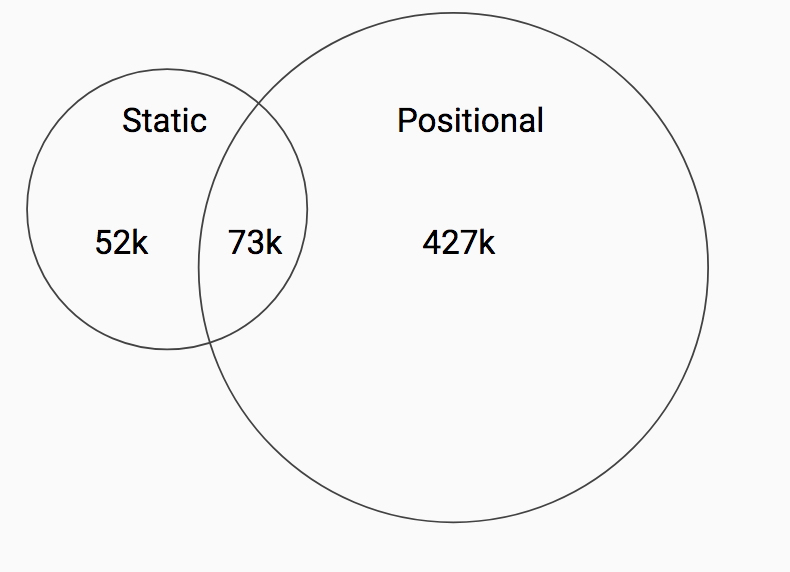
\includegraphics[width=0.5\textwidth]{images/ais_summary.png}
\caption{\label{fig:AIS broadcast summary}Number of positional and static AIS messages for a period of 1 year}
\end{figure}

\section{Modelling}

Here we describe an approach to use AIS data to identify at what points along their trajectory the vessels were fishing.

\subsection{Feature generation}

After discussions with domain experts, we came up with a list of features that might be good indicators of fishing behavior.
We generated features like distance from shore, port, day or night during the time of navigation etc. We then fit a Random Forest model to compute how each of the feature contributes towards the prediction.

\begin{figure}[H]
\centering
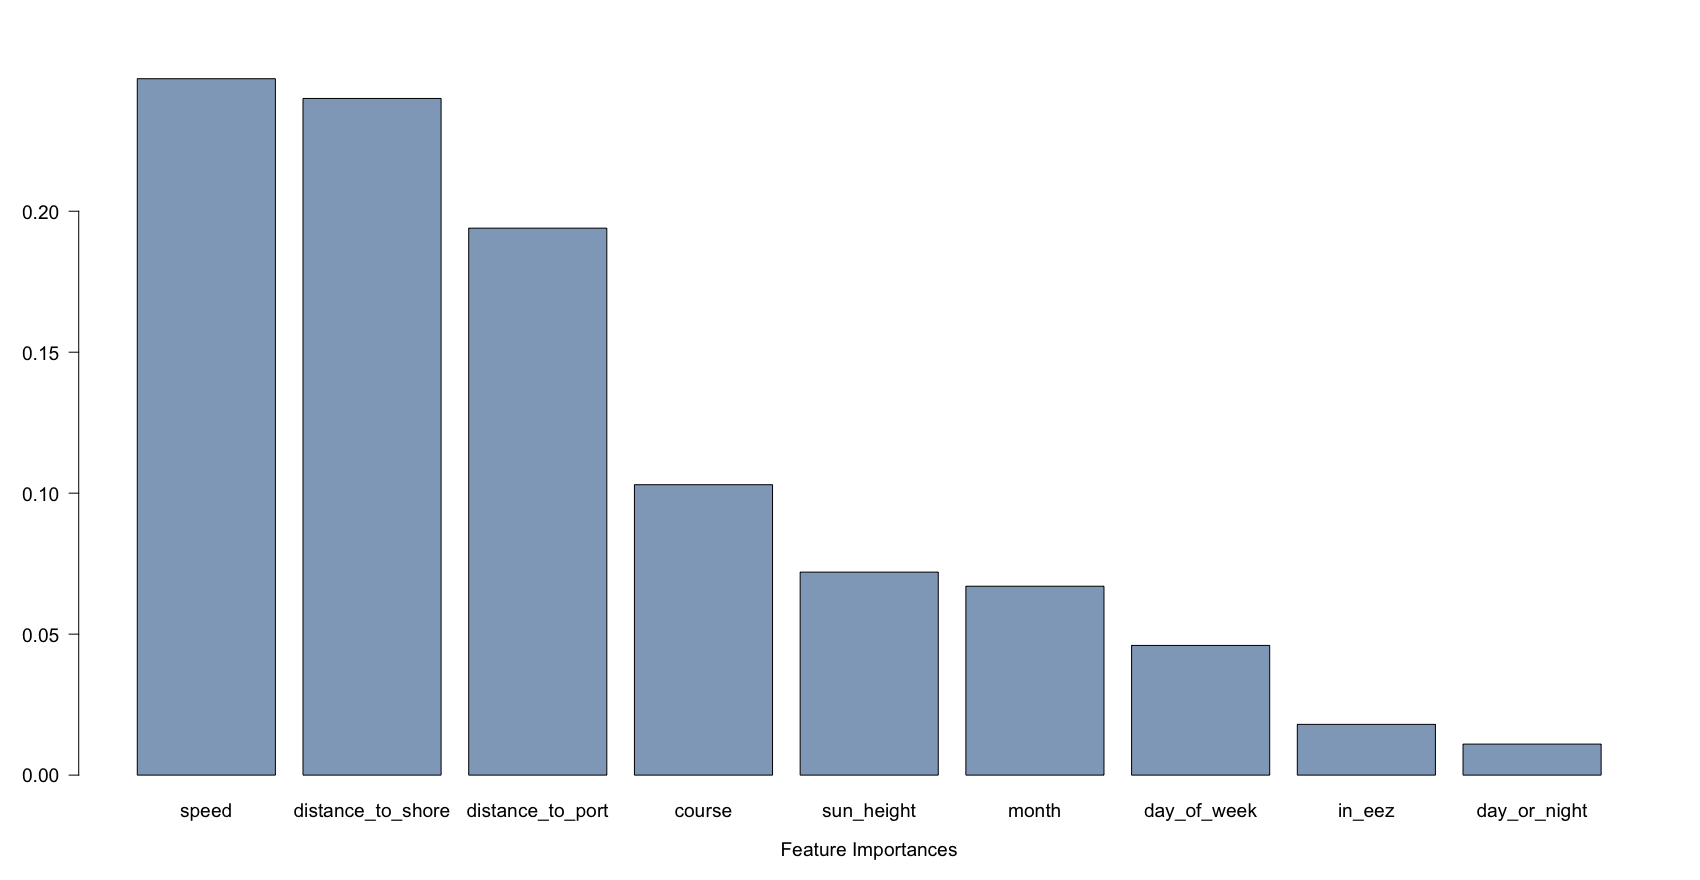
\includegraphics[width=0.5\textwidth]{images/feature_importance_final.png}
\caption{\label{fig:Feature importance}Feature importance for AIS positional features.}
\end{figure}

\subsection{Training and cross-validation}

Given we have a time series data, we split our data set into multiple temporal folds. For each fold, we split the train-test set as illustrated in the following figure.

\begin{figure}[H]
\centering
\includegraphics[width=0.5\textwidth]{images/temporal_cv.png}
\caption{\label{fig:Temporal Cross-validation}Temporal splits for each fold}
\end{figure}

We compute various metrics like precision, recall, false positive and true positives rates etc.

\subsection{Model selection}
After talking to our partners, we came to the conclusion that we want to optimize for precision of our models.
For example, in the following figure, you can see three precision-recall curves. For the model represented by the blue curve, you see high precision at first and then the precision get worse than the same for other models. The models we select also depend on how many cases our partner can act upon. If the partner can act upon K cases, then we should select the model that maximizes precision for those K cases.

\begin{figure}[H]
\centering
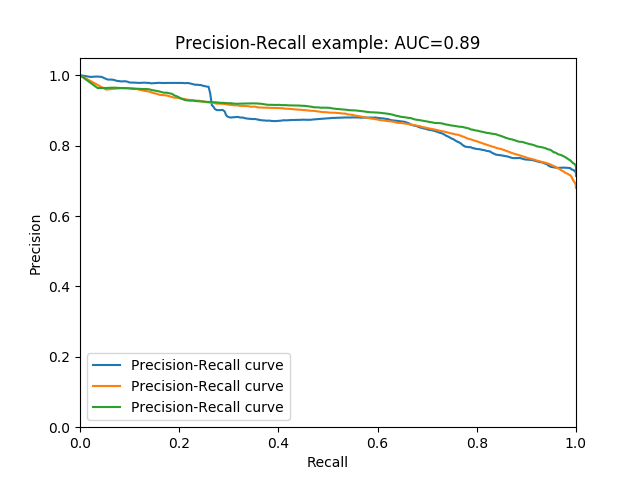
\includegraphics[width=0.5\textwidth]{images/precision_recall_curve.png}
\caption{\label{fig:Precision-Recall}Precision-Recall curve for different models}
\end{figure}

\section{Evaluation}

In the absence of a labeled prediction set, we are employing a few heuristics to examine the performance of our models.
For example, average fishing score for reported fishing vessels should in general, be greater than the same for vessels that don't report themselves as fishing.

	
Vessels spend most of their time being docked. Also, reported fishing vessels spend only a small fraction of their time actually fishing.

\begin{figure}[H]
\centering
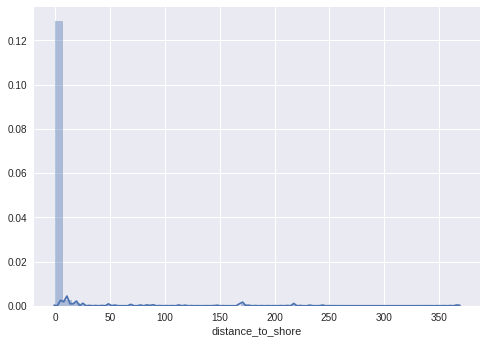
\includegraphics[width=0.5\textwidth]{images/distance_to_shore.png}
\caption{\label{fig:Distance to shore distribution}Distribution of distance to shore in the AIS messages}
\end{figure}


\begin{figure}[H]
\centering
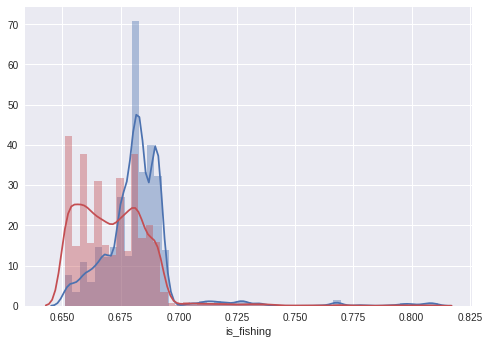
\includegraphics[width=0.5\textwidth]{images/fishing_score_distributions.png}
\caption{\label{fig:Fishing score distribution}Fishing score distributions for reported and non reported fishing vessels.}
\end{figure}


\bibliographystyle{alpha}
\bibliography{sample}

\end{document}
 % approach
\subsection{Intersection AIS and Satellite imagery}

Marine traffic detection using remote sensing approach is a commonly addressed task. \citeA{Brusch2011} showed how 
AIS and Synthetic Aperture Radar (SAR) data could be used in conjunction to detect vessels in small portions where
the satellite imagery tiles contain positional AIS messages. \citeA{Corbane2008} follow a similar approach joining
Vessel Monitoring System (VMS) and commercial satellite imagery to identify common features of shrimp boats. Although
these endeavors are working solutions, there is still wanting a strategy that can bring different sources of data that
can complement SAR data. One of these possible sources of data is high-resolution imagery, which until now has been 
restricted to commercial use only \cite{Greidanus2006}.

Our approach follows the work previously outlined since it is combining positional GPS data with remote sensing data. 
Nonetheless, it departs from it since it is mainly focused on UII activities, and also uses worldwide satellite imagery 
and AIS positional data. This work, at least in this preliminary stage, can work to create a comprehensive image 
database that can serve ultimately to validate the AIS data accuracy, and also the feasibility of joining different 
data sources to understand risky behaviors related to UII. 

The process of image retrieval was a tree step operation. First, we retrieve all the available images in \textit{Marine Areas} and
\textit{Ocean Areas} for our time frame (May 2016 to June 2017). The former are defined as areas is open waters; meanwhile the latter
are the areas near the continental land. This process yielded 187.038 images.\footnote{Additional 18.476 images were retrieved using 
Planet imagery only for the Torres Strait.}. Second, we overlap the bounding boxes of the imagery tiles with the AIS positional signals. 
This process was not only a spatial join, but also a time join which took into account the difference of time between the picture 
capture timestamp and the positional AIS timestamp. Figure \ref{overlap} shows the outcome of this step. In total, for Digital Globe,
the intersection retrieved 1.072 AIS positional signals (487 unique vessels). Third, we crop the images using a 800 meters square buffer 
of each the AIS coordinates inside the overlap. The Figure \ref{mosaic} shows the final outcome of this process.

\begin{figure}[h]
	\centering \caption{Overlap Digital Globe and AIS data (May 2016 - June 2017)}\label{overlap}
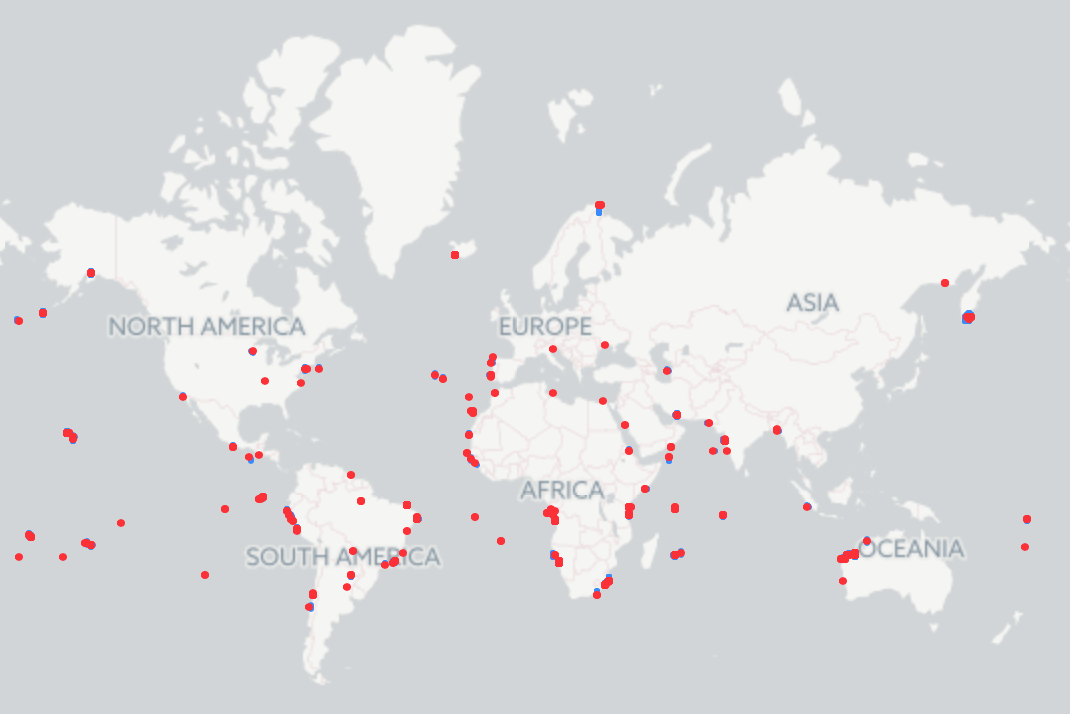
\includegraphics[width=0.6\linewidth]{images/overlap_gbdx.png} 
\begin{flushleft}
\rule{1.2in}{0em} \scriptsize Source: Digital Globe, Spire and OpenStreetMap. \\
\par
\end{flushleft}
\end{figure}

\begin{figure}[h]
	\centering \caption{Cropped  (May 2016 - June 2017)}\label{overlap}
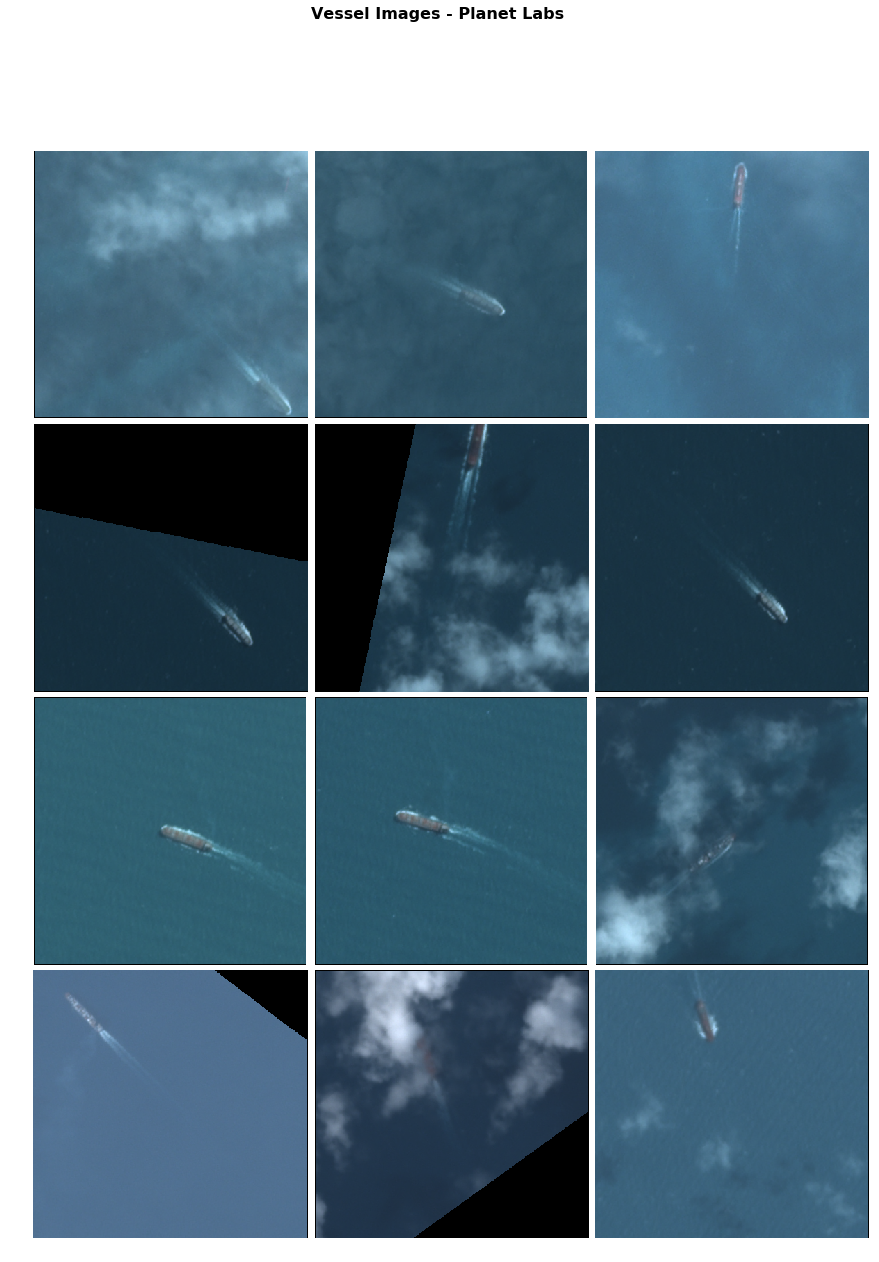
\includegraphics[width=0.6\linewidth]{images/mosaic_planet_torres_strait.png} 
\begin{flushleft}
\rule{1.2in}{0em} \scriptsize Source: Planet and Spire. \\
\par
\end{flushleft}
\end{figure}


 % sat_imagery
\section{Evaluation methodology}
evaluate this
 % evaluation
\section{Future work}
Lots will be done in the future
 % further work
\section*{Acknowledgement}
The authors would like to thank x, y, and z for their dedication.


\newpage
\printglossaries
%\printglossary[type=\acronymtype]
%\printglossary[type=main]


\bibliography{bibliography}
\bibliographystyle{ieeetr}

\end{document}
